\documentclass{beamer}

\usetheme{AnnArbor}

\title{Milkymist SoC}
\subtitle{A performance-driven SoC architecture for video synthesis}
\author{S\'ebastien Bourdeauducq}
\institute{KTH}
\date{June 2010}

\begin{document}

\frame{
  \begin{figure}[H]
  
\includegraphics[height=20mm]{newlogo.eps}
  \end{figure}
  \titlepage
}

\section{Introduction}
\subsection{How it all started}
\frame
{
  \frametitle{How it all started}
A device for video performance artists (VJs)...
  \begin{itemize}
  \item inspired by the popular MilkDrop program for PCs
  \item with many interfaces: MIDI, DMX, video in
  \item highly integrated
  \end{itemize}

At the frontier between...
  \begin{itemize}
  \item big computers with software to render visual effects
  \item and small, handy microcontroller boards you connect to anything
  \end{itemize}
}

\frame
{
  \frametitle{How does MilkDrop look?}
  \begin{figure}[H]
  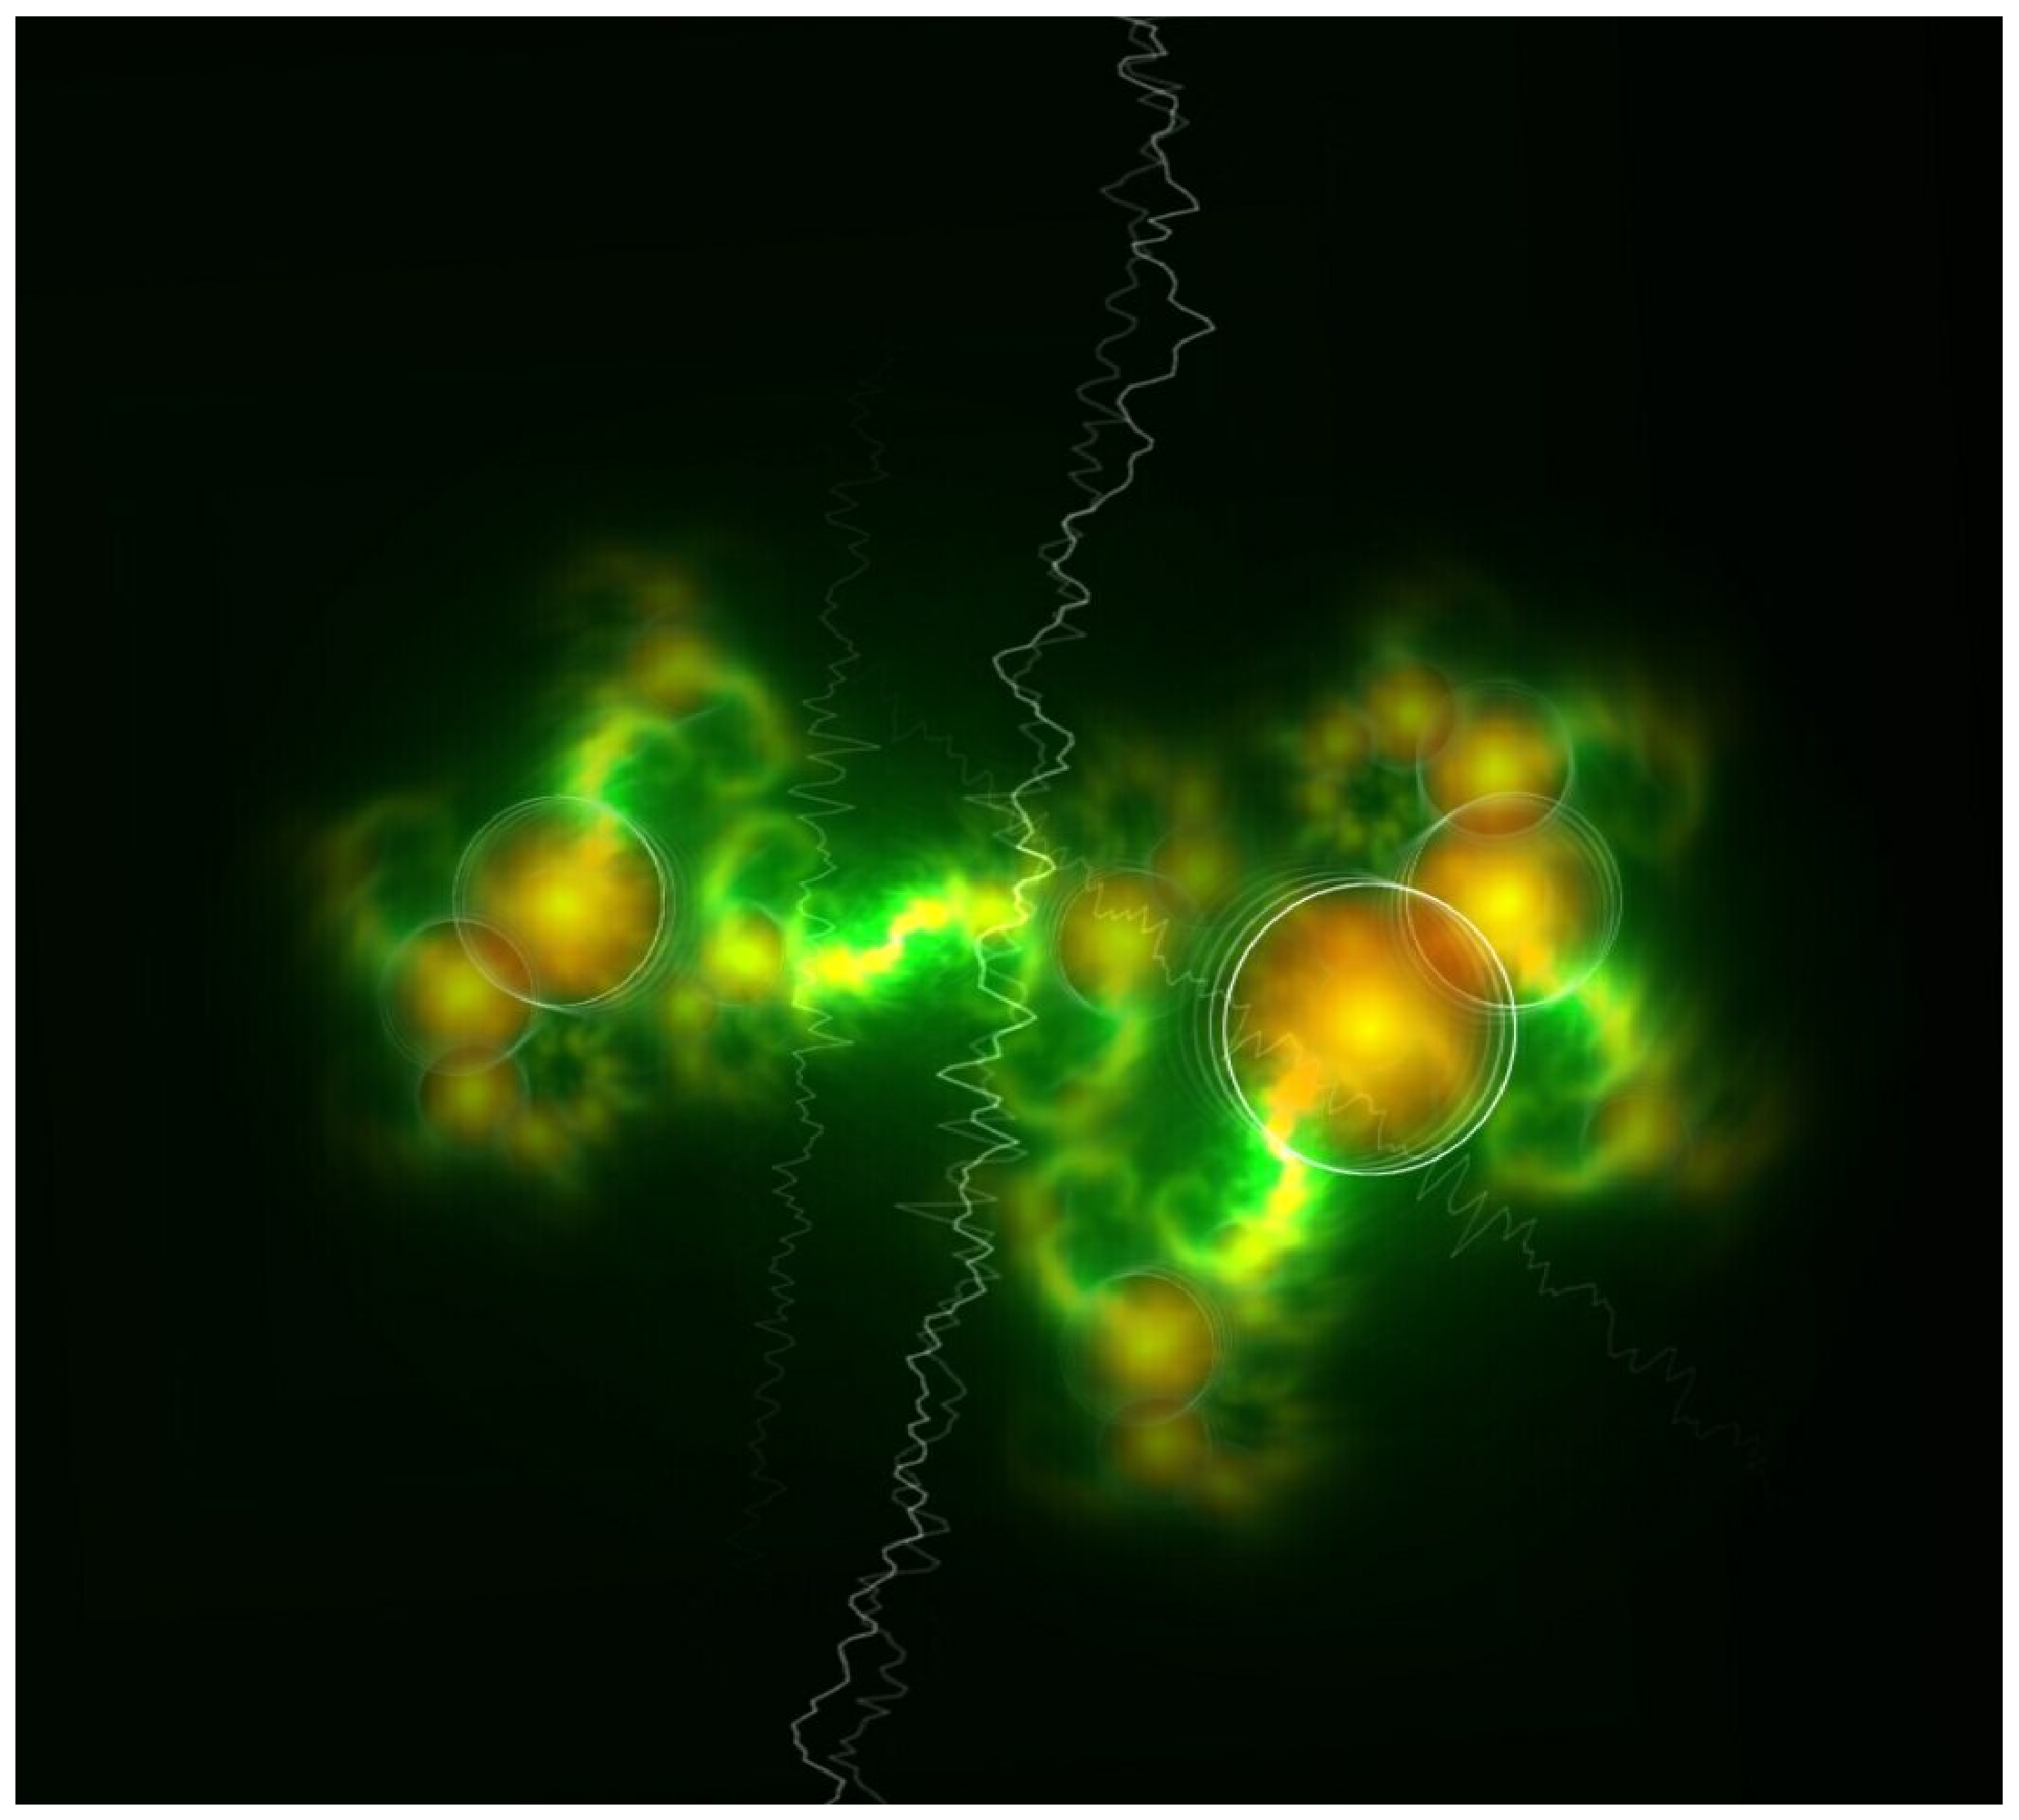
\includegraphics[height=58mm]{milkdrop1.eps}
  \end{figure}
}

\frame
{
  \frametitle{How does MilkDrop look?}
  \begin{figure}[H]
  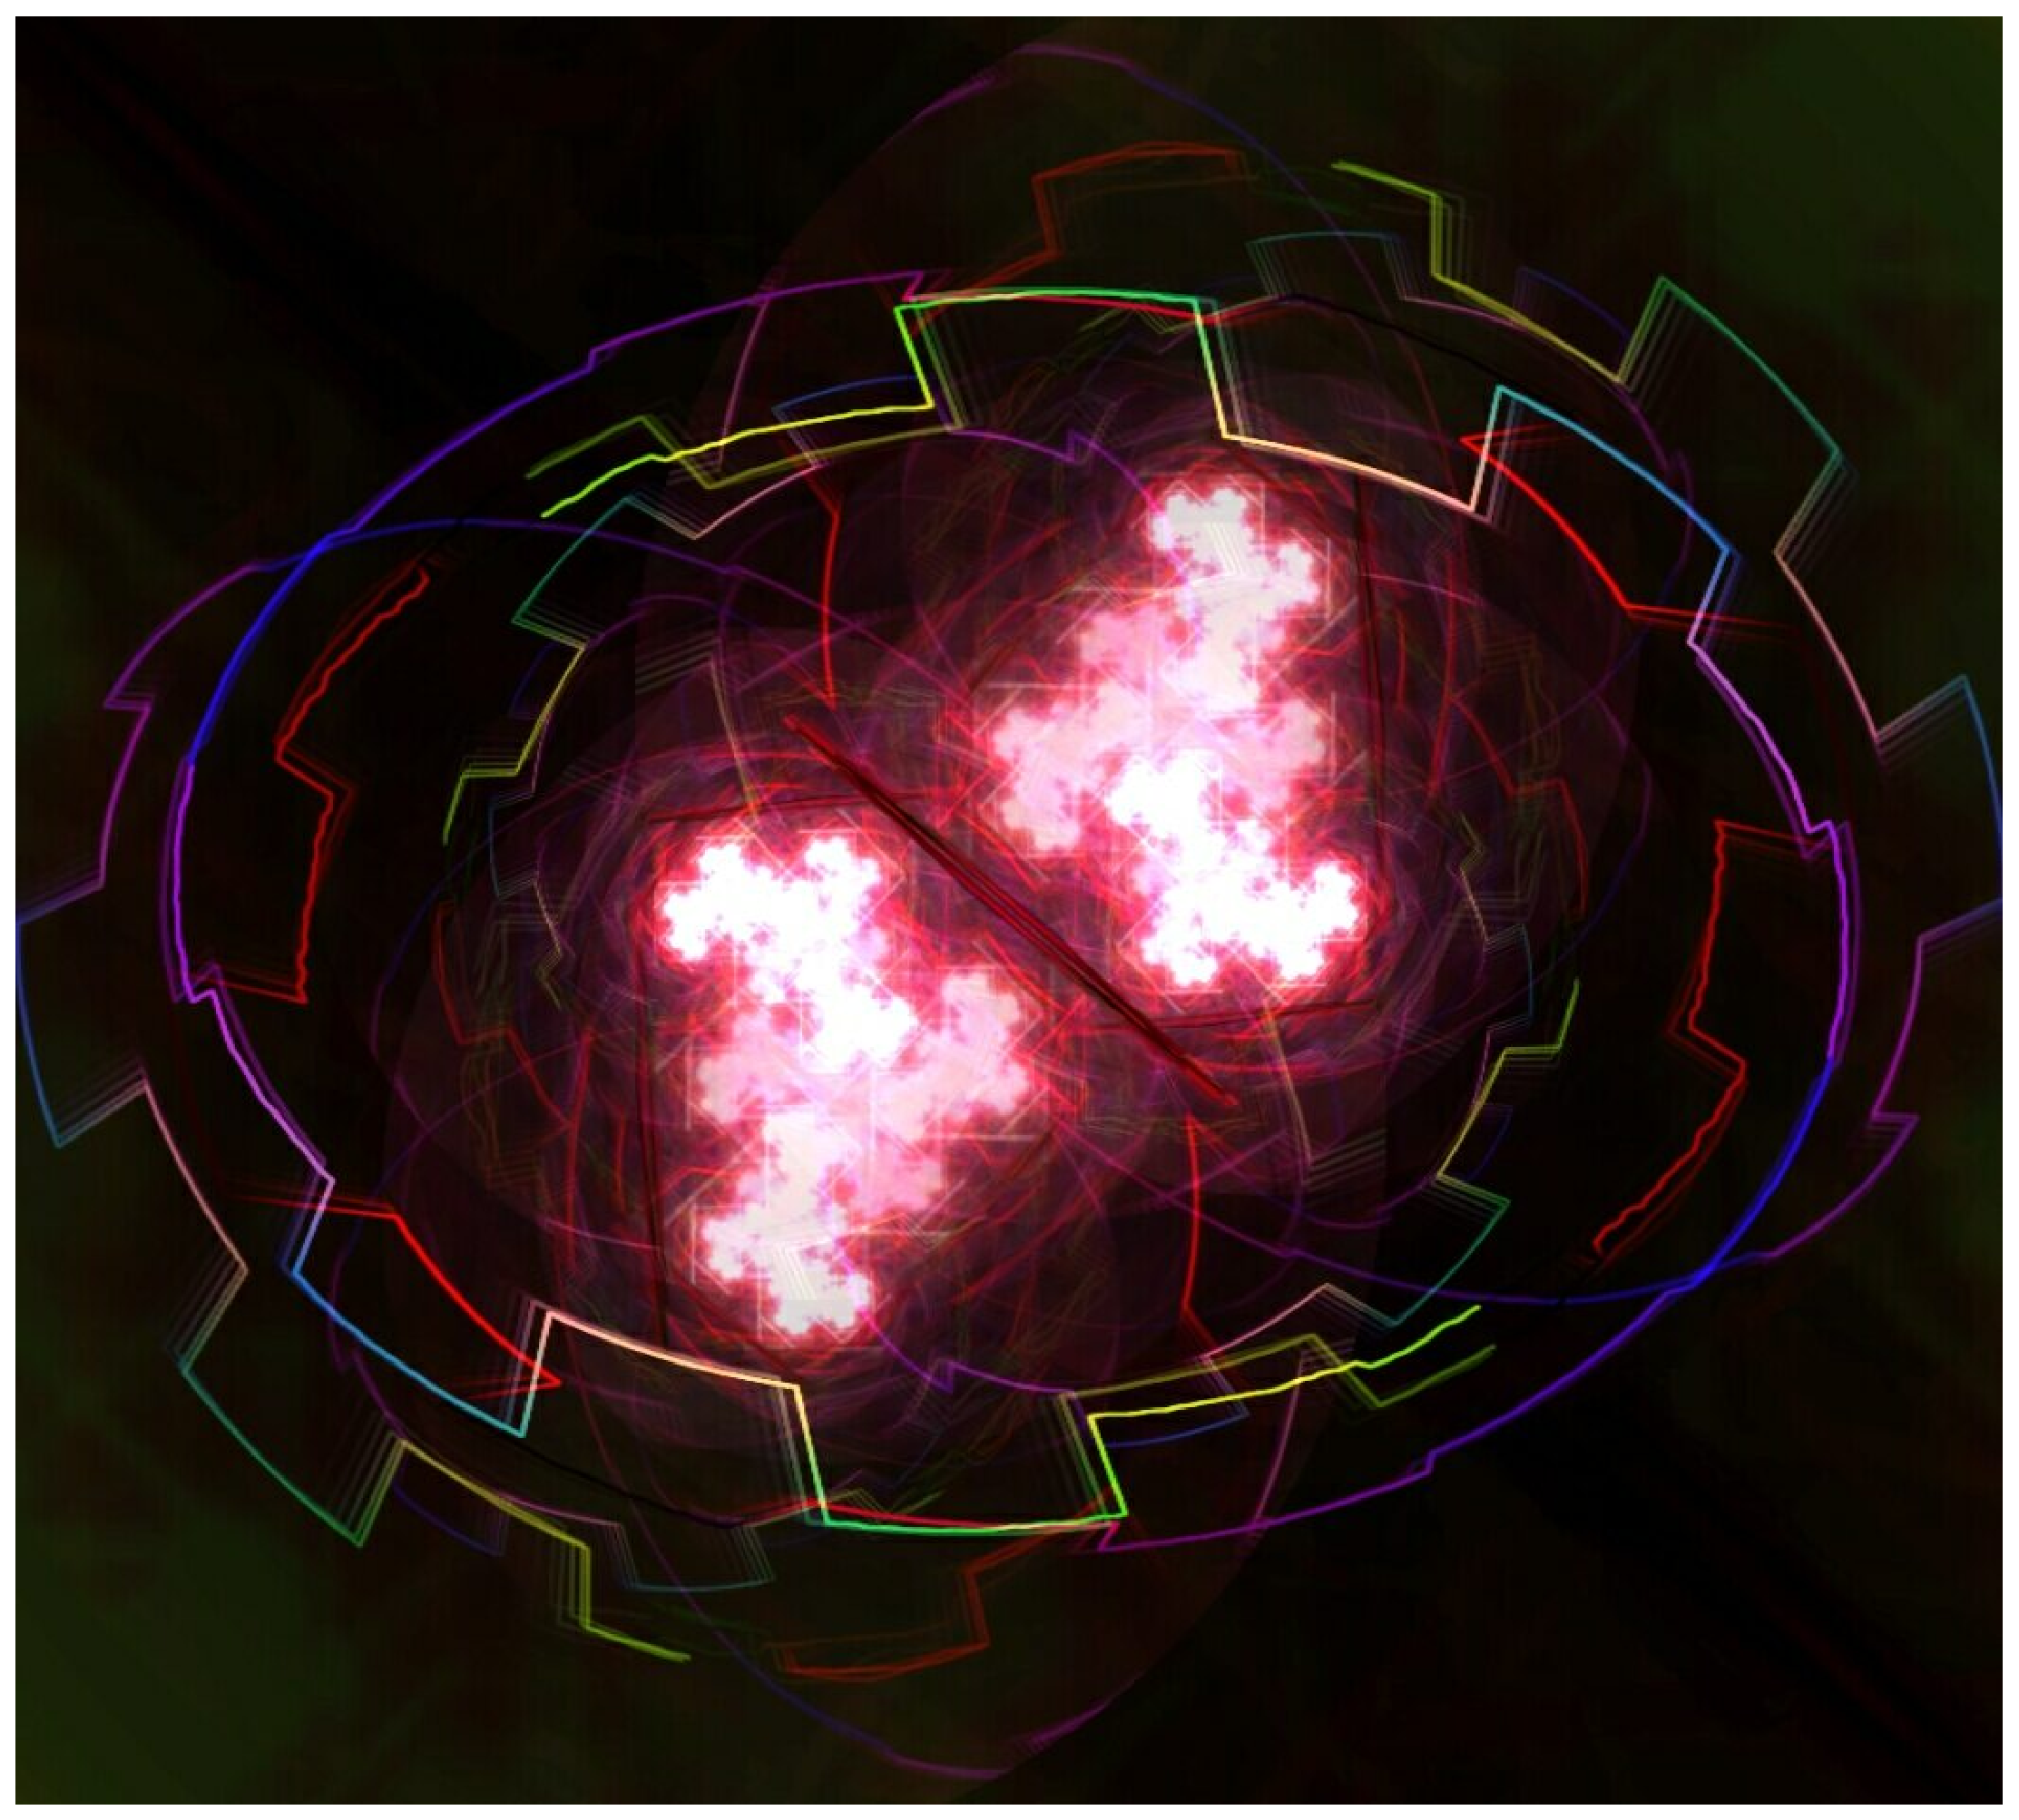
\includegraphics[height=58mm]{milkdrop2.eps}
  \end{figure}
}

\frame
{
  \frametitle{How does MilkDrop look?}
  \begin{figure}[H]
  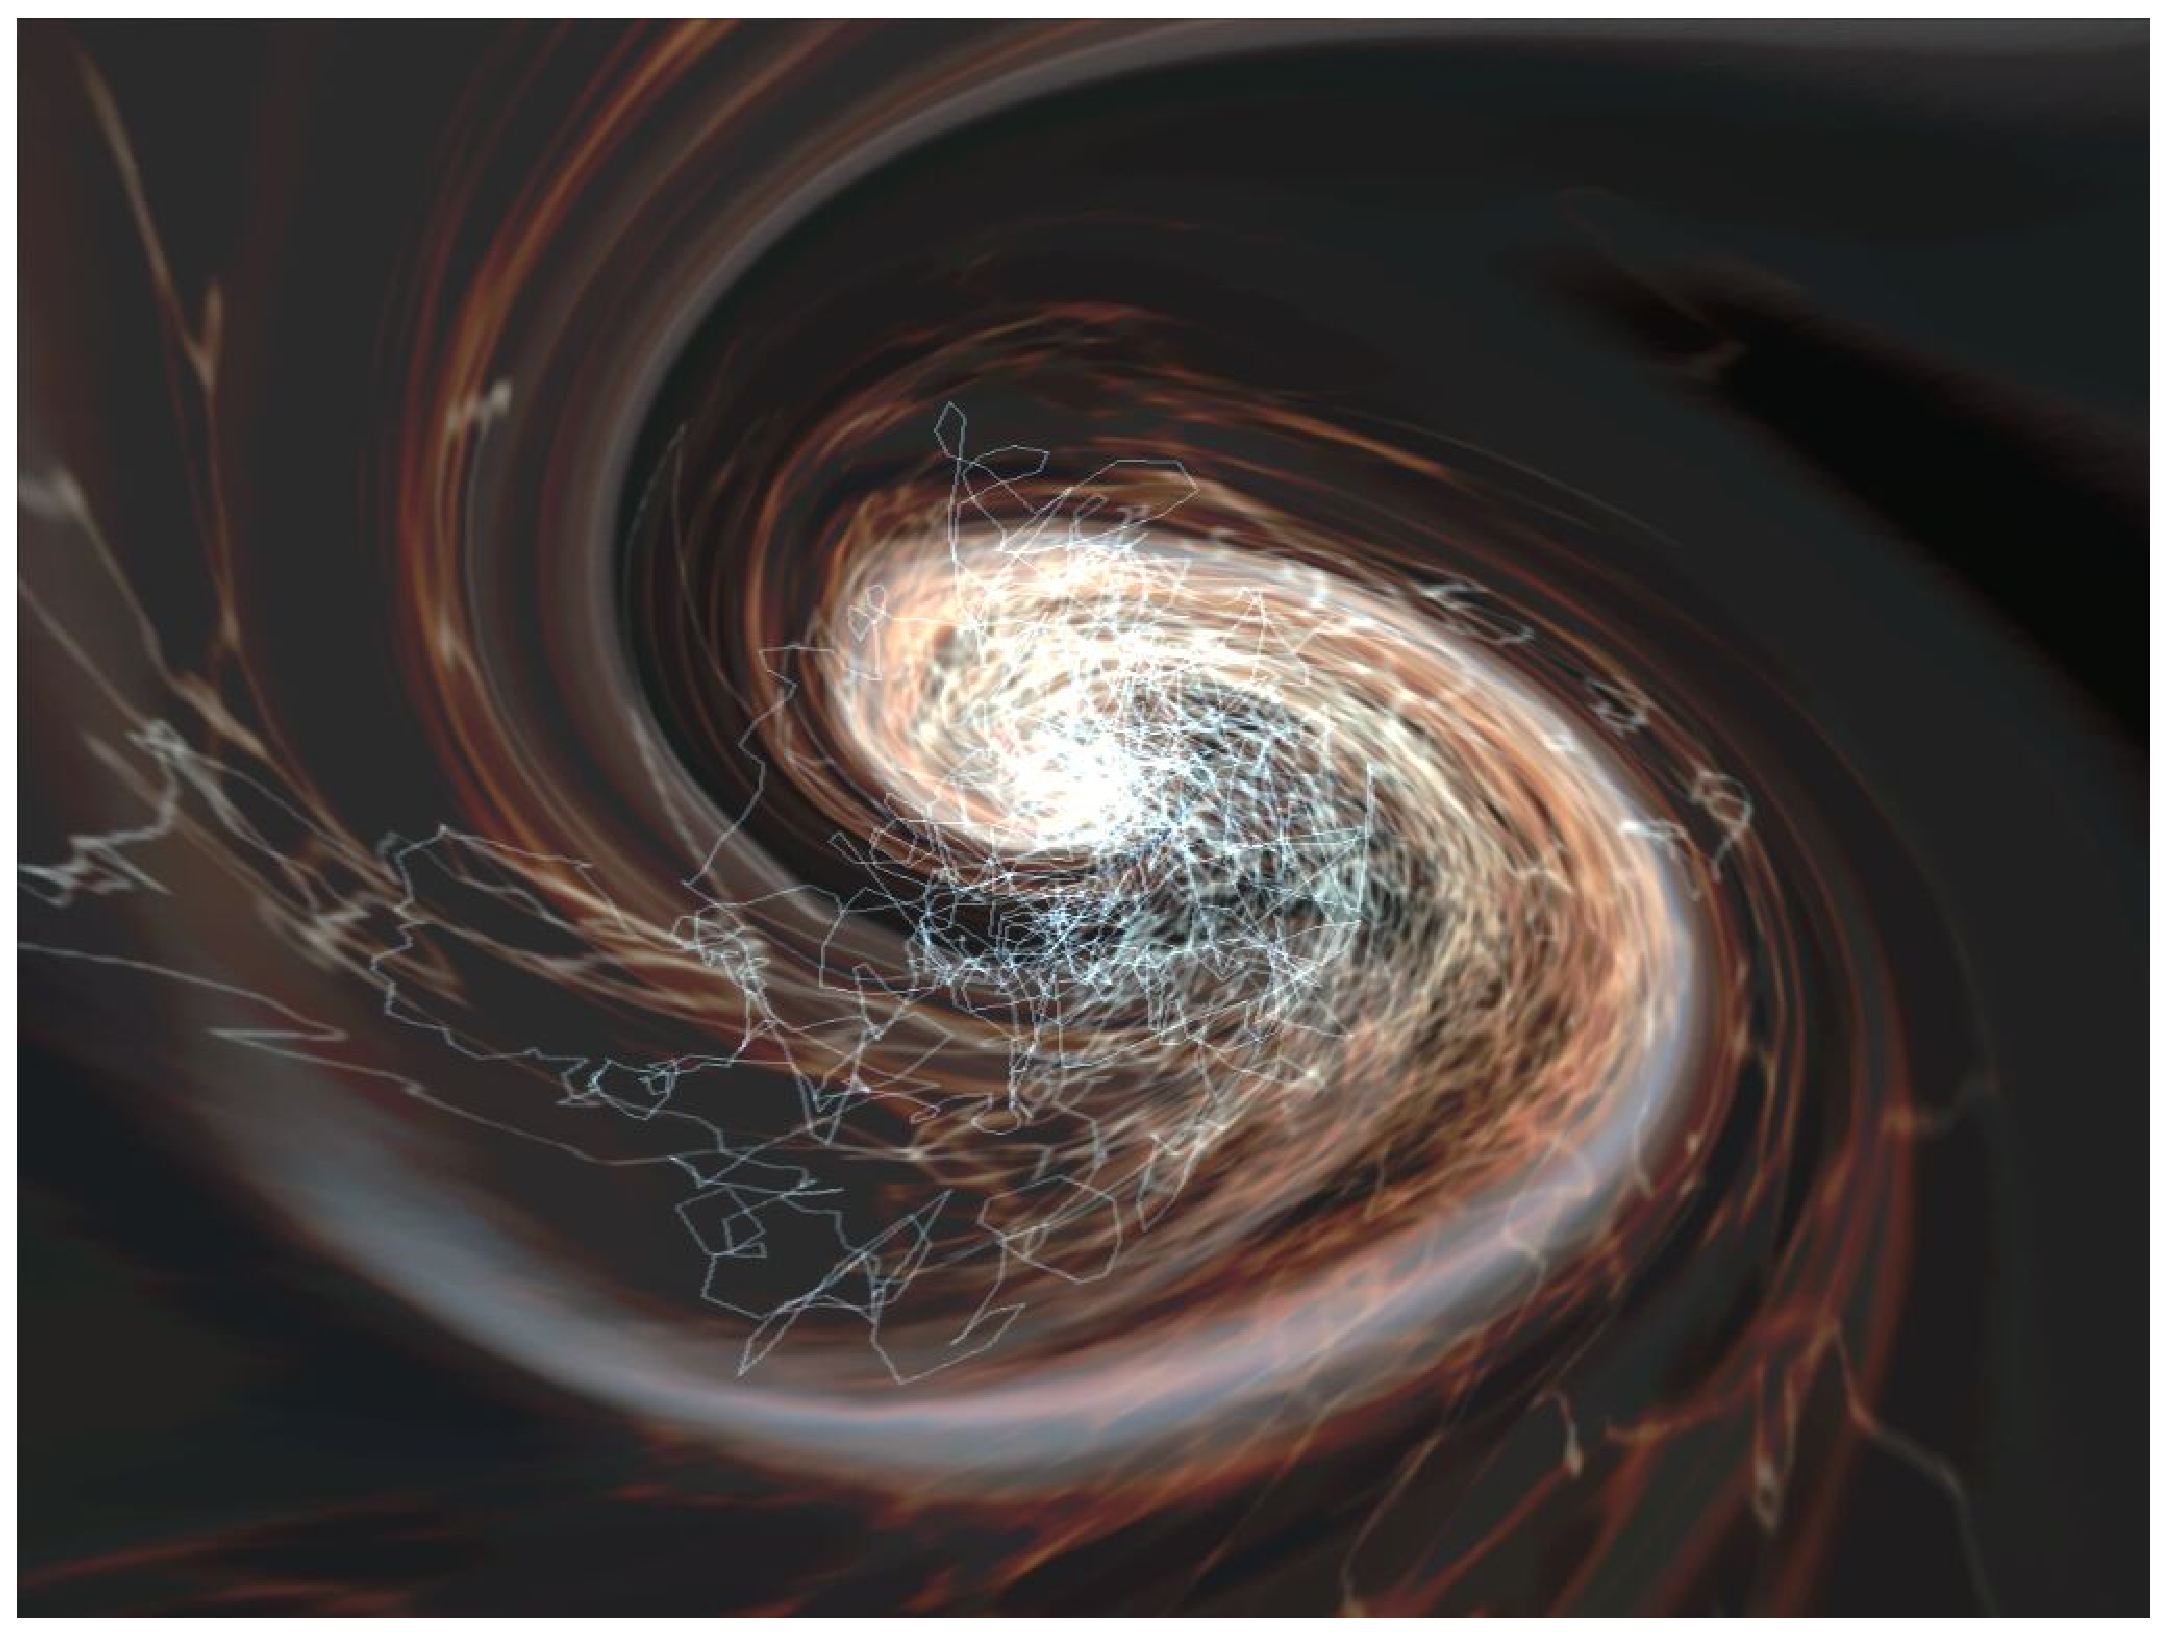
\includegraphics[height=58mm]{milkdrop3.eps}
  \end{figure}
}

\subsection{How does MilkDrop work?}
\frame
{
  \frametitle{How does MilkDrop work?}

In two words:
  \begin{itemize}
  \item Take the current image, and distort it
  \begin{itemize}
    \item zoom
    \item rotation
    \item scaling
    \item others...
  \end{itemize}
  \item Draw waves and shapes
  \item Display the result
  \item Repeat the process (iterative rendering)
  \end{itemize}
}

\frame
{
  \frametitle{How does MilkDrop work?}

  \begin{itemize}
  \item Distortion and waves are controlled by fully customizable equations
  \item The set of those equations is called a ``preset'' or ``patch''
  \item Interaction of the visuals with sound is defined by those equations
  \item ...and also with DMX and MIDI in Milkymist
  \end{itemize}
}

\subsection{Challenges}
\frame
{
  \frametitle{Challenges}

  \begin{itemize}
  \item The need for a CPU
  \begin{itemize}
     \item flexibility
     \item ease of reprogramming, patching software bugs
     \item software-friendly tasks: GUI, filesystems, protocols, ...
  \end{itemize}
  \item Speed, size, and cost
  \begin{itemize}
     \item careful design
     \item balance between hardware and software
     \item software is cheap and slow, hardware is expensive and fast
  \end{itemize}
  \item Memory problems: bandwidth, size
  \item Compute-intensive operations
  \begin{itemize}
     \item distorting the image
     \item evaluating the equations
  \end{itemize}
  \end{itemize}
}

\subsection{SoC platform}
\frame
{
  \frametitle{SoC platform}

  \begin{itemize}
  \item What is needed is a SoC with graphics acceleration
  \item They are ubiquitous today
  \begin{itemize}
  \item Texas Instruments OMAP
  \item Freescale i.MX
  \end{itemize}
  \item However, those are closed and proprietary
  \item This work: a new open source SoC that can run MilkDrop
  \end{itemize}
}


\section{Memory subsystem}
\subsection{The memory problem}
\frame
{
  \frametitle{The memory problem}

  \begin{itemize}
  \item A tough one.
  \item The application requires memory to be large, fast, and cheap.
  \item The required memory size prohibits the use of SRAM
  \item ...then we have to use DRAM and face all its problems.
  \end{itemize}
}

\frame
{
  \frametitle{Bandwidth estimation}

  \begin{tabular}{|l|l|}
  \hline
  \textbf{Task} & \textbf{Required bandwidth} \\
  \hline
  VGA frame buffer & 950Mb/s \\
  \hline
  Distortion & 250Mb/s \\
  \hline
  Live video & 300Mb/s \\
  \hline
  Scaling & 500Mb/s \\
  \hline
  Video echo & 900Mb/s \\
  \hline
  NTSC input & 200Mb/s \\
  \hline
  Software and misc. & 200Mb/s \\
  \hline
  \textbf{Total} & \textbf{3.3Gb/s} \\
  \hline
  \end{tabular}\\

  \begin{itemize}
  \item One DDR SDRAM chip running at 100MHz:
  \begin{itemize}
  \item 3.2Gbps \underline{peak bandwidth}
  \item 32MB capacity
  \item a few dollars
  \end{itemize}
  \end{itemize}
}

\subsection{Optimizing memory performance}
\frame
{
  \frametitle{Peak bandwidth?}

  Performance of SDRAM depends a lot on the cleverness of its controller. Simplified example:

  \begin{figure}[H]
  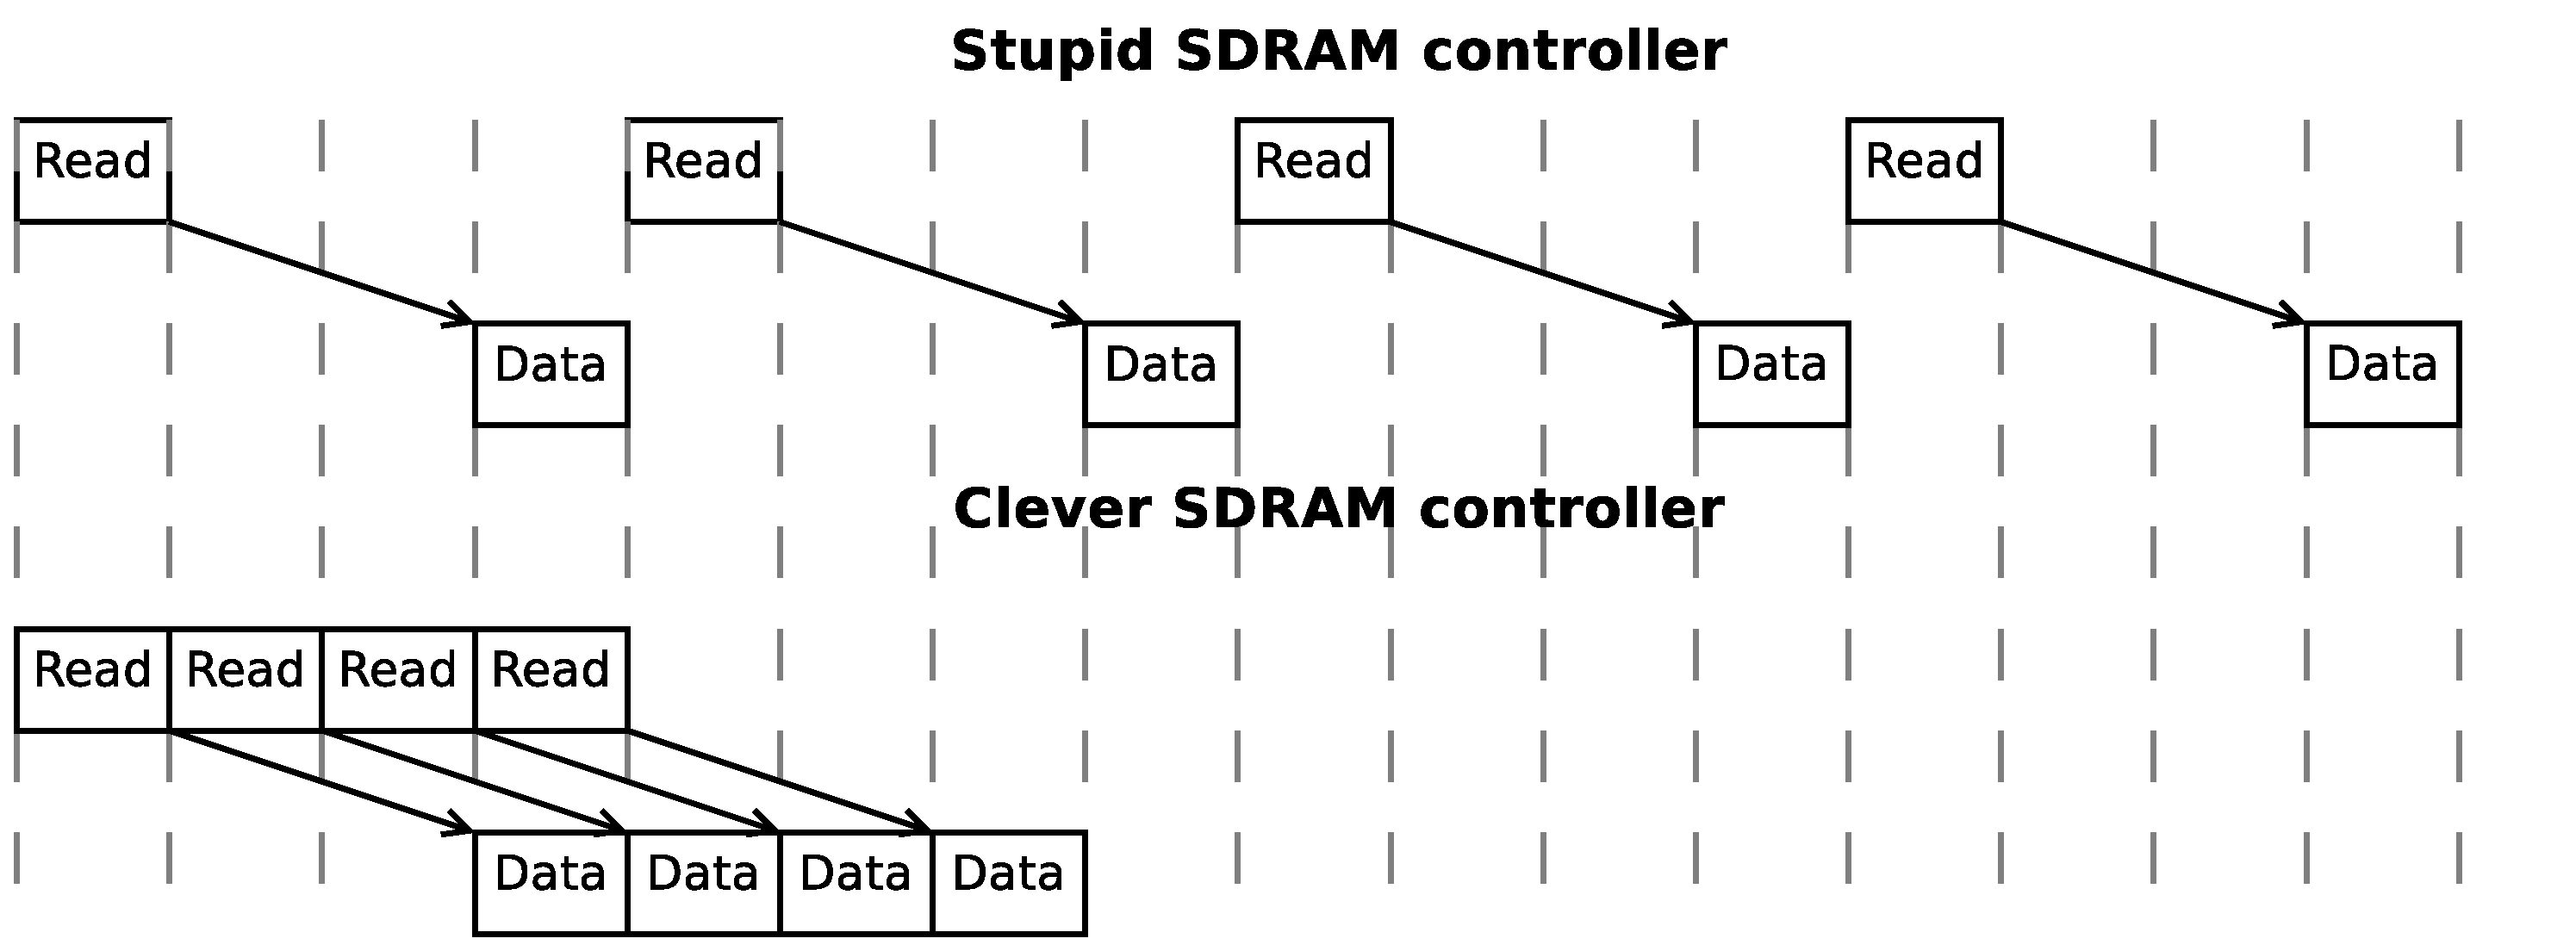
\includegraphics[height=30mm]{memlatency.eps}
  \end{figure}

  In Milkymist, memory transfers are always done using bursts of 4 consecutive words. The bus master caches or discards the data it does not want.
}

\frame
{
  \frametitle{Techniques used in Milkymist}
  \begin{itemize}
  \item Single SDRAM and system clock domains (reduces latency)
  \item Bursts
  \item Critical word first
  \item Pipelining
  \item Page mode DRAM control
  \end{itemize}
}

\frame
{
  \frametitle{Bursts: a good heuristics?}

  \begin{itemize}
  \item Good for the VGA framebuffer (a big bandwidth consumer):
  \begin{itemize}
  \item when it gets a burst of consecutive chunks from memory...
  \item those chunks also represent consecutive pixels (in scan order)
  \item ...so it can just put them in its output FIFO and easily acheive 100\% utilization!
  \end{itemize}
  \item It is the same for video inputs.
  \item For image distortion: yes; more on this later.
  \item For software: principle of temporal/spatial locality, caches.
  \end{itemize}
}

\subsection{Results}
\frame
{
  \frametitle{Our memory system}

  \begin{figure}[H]
  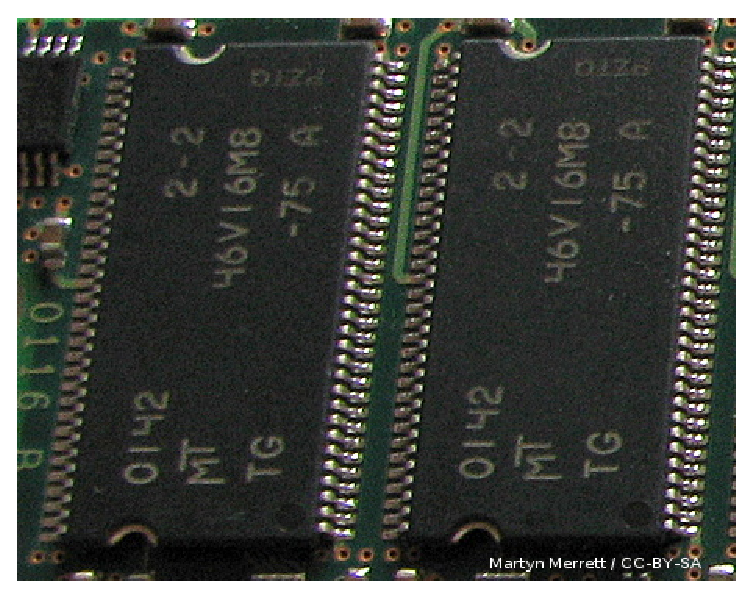
\includegraphics[height=35mm]{ddr64.eps}
  \end{figure}

  \begin{itemize}
  \item 2 chips of 32-bit DDR SDRAM at 100MHz
  \item Peak bandwidth of 6.4Gbps
  \item Oversized -- but this is necessary
  \end{itemize}
}

\frame
{
  \frametitle{Performance measurement}

  \begin{tabular}{|l|l|l|l|}
  \hline
  \textbf{Patch} & BW & AMAT & Max. BW bound \\
  \hline
  Idle & 292 & 5.51 & 3932 \\
  \hline
  Bright Fiber Matrix 1 & 990 & 6.37 & 3474 \\
  \hline
  Swirlie 3 & 1080 & 6.71 & 3320 \\
  \hline
  Spacedust & 1021 & 6.47 & 3427 \\
  \hline
  Snowflake Delight & 1399 & 6.28 & 3516 \\
  \hline
  Balk Acid & 1427 & 6.38 & 3469 \\
  \hline
   \end{tabular}
}


\section{Distorting the image}
\subsection{Presentation}
\frame
{
  \frametitle{What is ``distortion''?}

  \begin{figure}[H]
  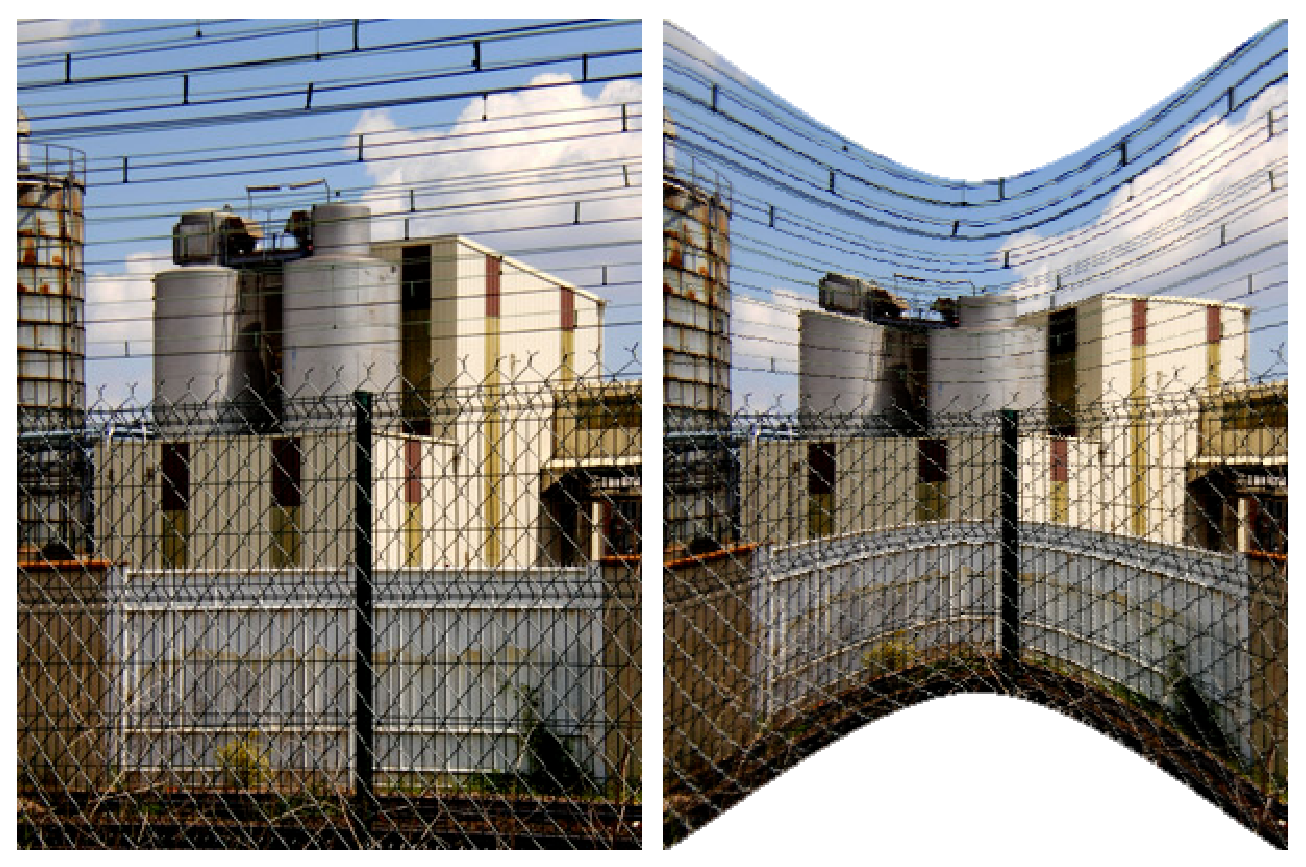
\includegraphics[height=40mm]{distortionsanofi.eps}
  \end{figure}
}

\frame
{
  \frametitle{More precisely...}
  \begin{itemize}
  \item Tessellate the source image with rectangles.
  \item Compute the source (texture) coordinates on each vertex.
  \item Fill each rectangle in the destination picture.
  \item Interpolate linearly the source (texture) coordinates.
  \item This is called \textit{texture mapping}.
  \end{itemize}
}

\subsection{Speed considerations}
\frame
{
  \frametitle{Speed constraints}

  \begin{itemize}
  \item Good system performance: must fill $> 31$ million pixels per second.
  \item With a 100MHz clock, we have $< 3.2$ cycles to put out a pixel.
  \item Precludes any software implementation (more than 40 times too slow).
  \end{itemize}
}

\frame
{
  \frametitle{Solutions}

  \begin{itemize}
  \item Efficient algorithm
  \begin{itemize}
  \item Inspired by Bresenham's linear interpolation algorithm
  \end{itemize}
  \item ``SIMD'' parallelism
  \begin{itemize}
  \item the same operation on independent data can be done in parallel
  \item example: computing the interpolated X and Y in the texture
  \end{itemize}
  \item Pipelined parallelism
  \begin{itemize}
  \item Milkymist's TMU has about 20 pipeline stages
  \end{itemize}
  \item Smart memory access
  \begin{itemize}
  \item cache
  \item write buffer
  \end{itemize}
  \end{itemize}
}

\subsection{Cache}
\frame
{
  \frametitle{Using a cache}

  Example: rotation of a rectangle.
  \begin{figure}[H]
  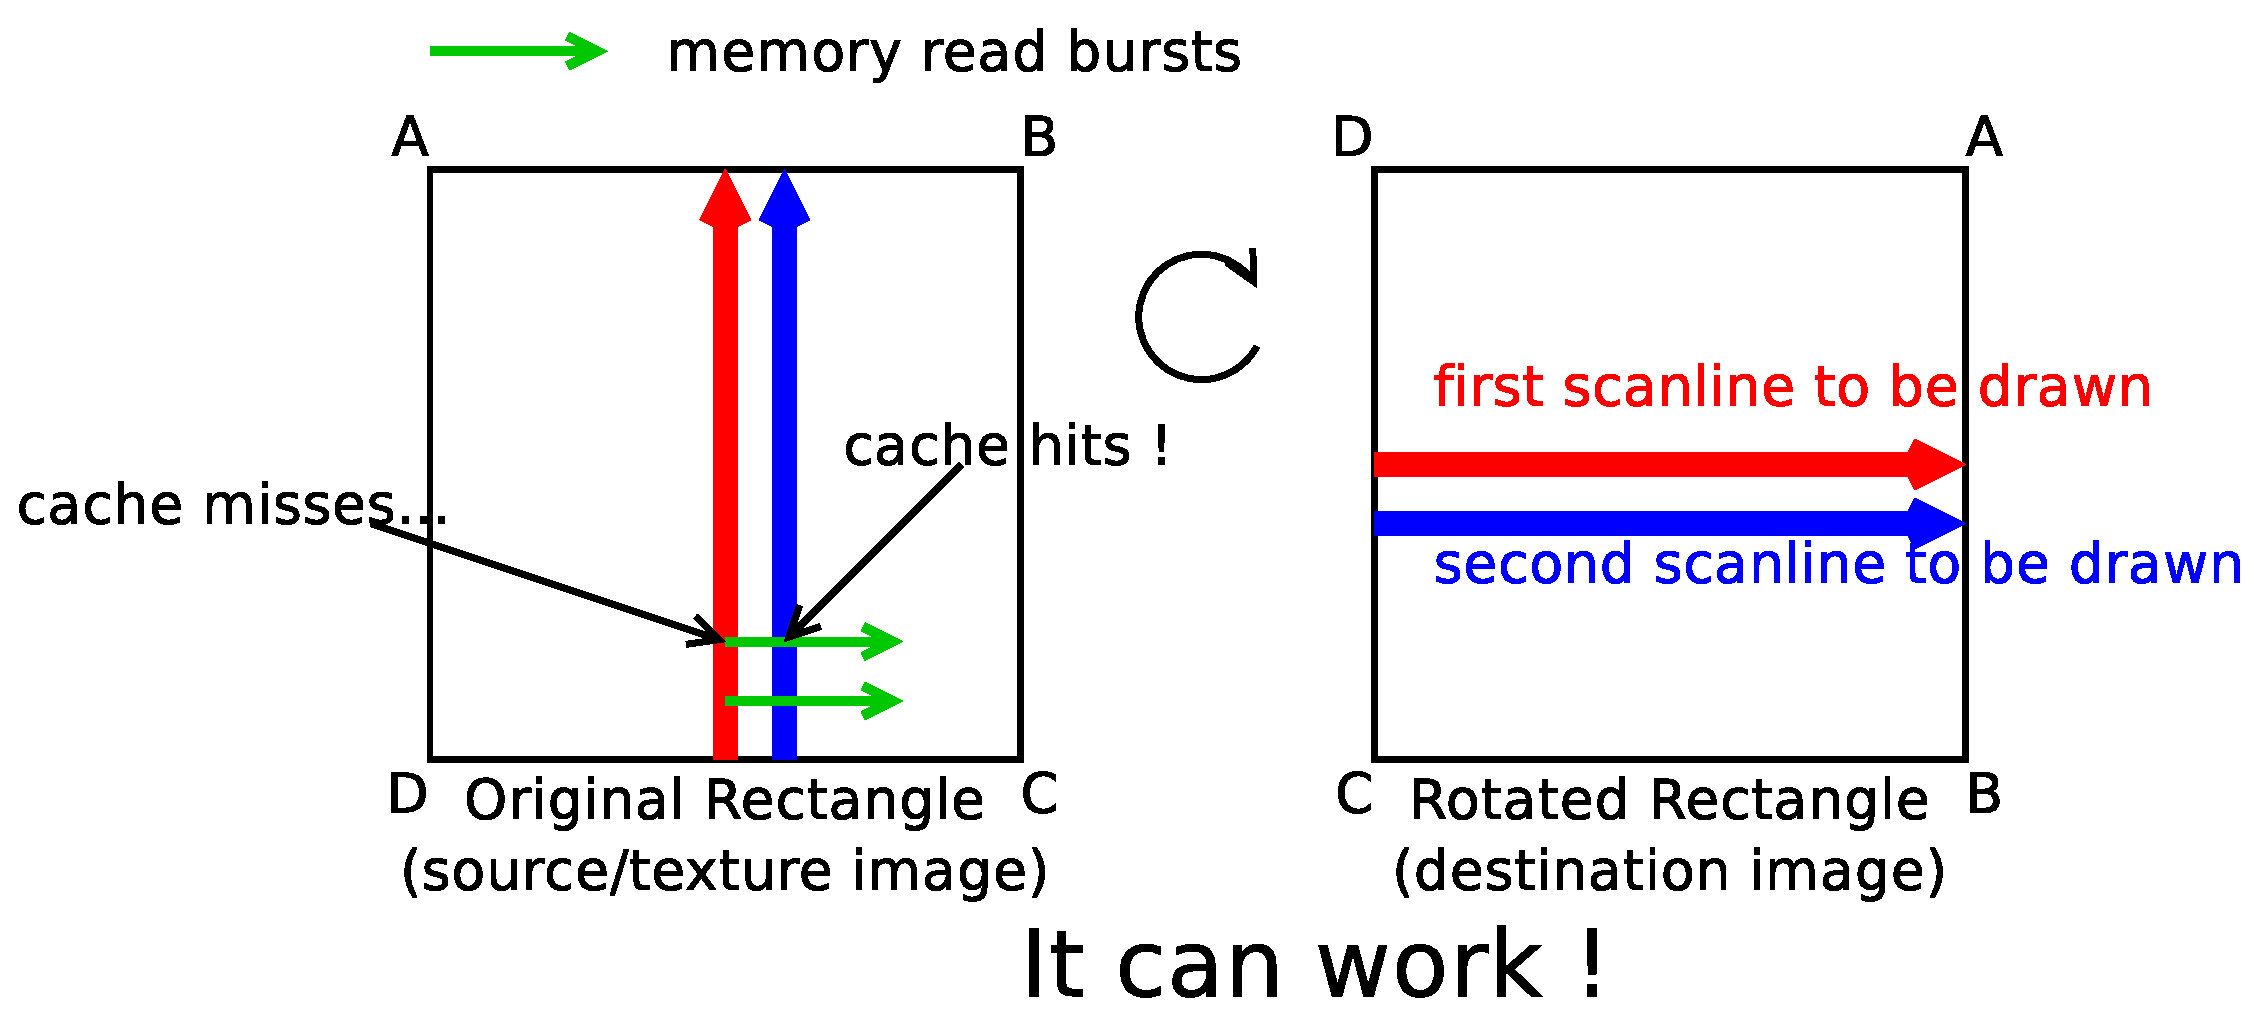
\includegraphics[height=40mm]{fillmempattern.eps}
  \end{figure}
}

\frame
{
  \frametitle{How big should the cache be?}
  \begin{itemize}
  \item Simulation with different sets of texture coordinates:
  \end{itemize}
  \begin{figure}[H]
  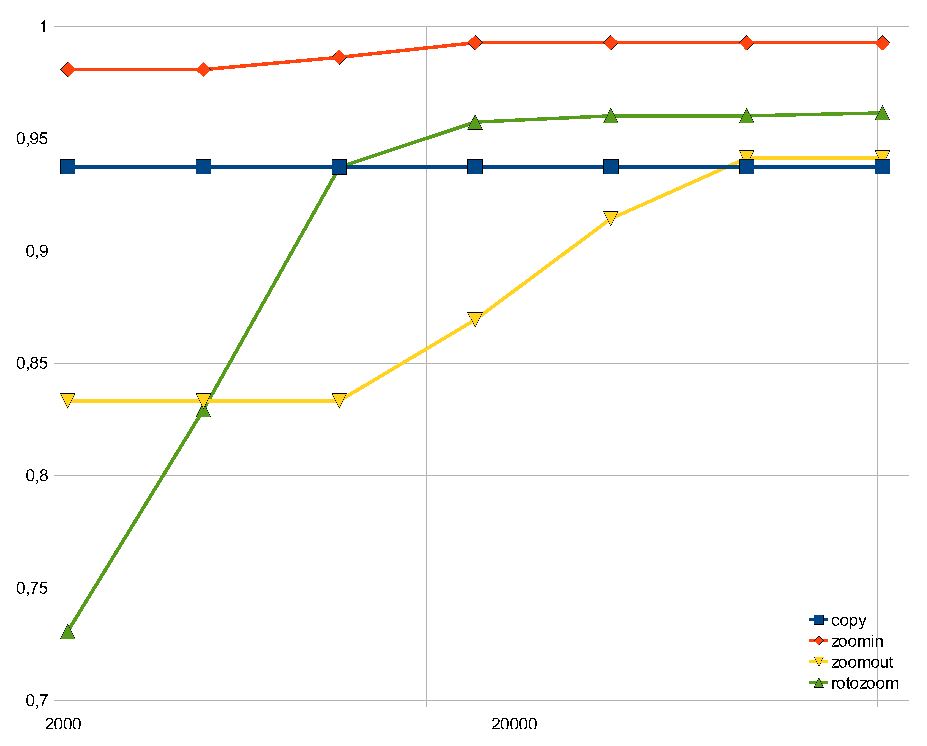
\includegraphics[height=55mm]{tcresultsgraph.eps}
  \end{figure}
}

\subsection{Write buffer}
\frame
{
  \frametitle{Write buffer}
  \begin{itemize}
  \item ``Double buffering'', stores two bursts.
  \item 1 pixel/clock up to 12 cycles of memory access time.
  \end{itemize}
  \begin{figure}[H]
  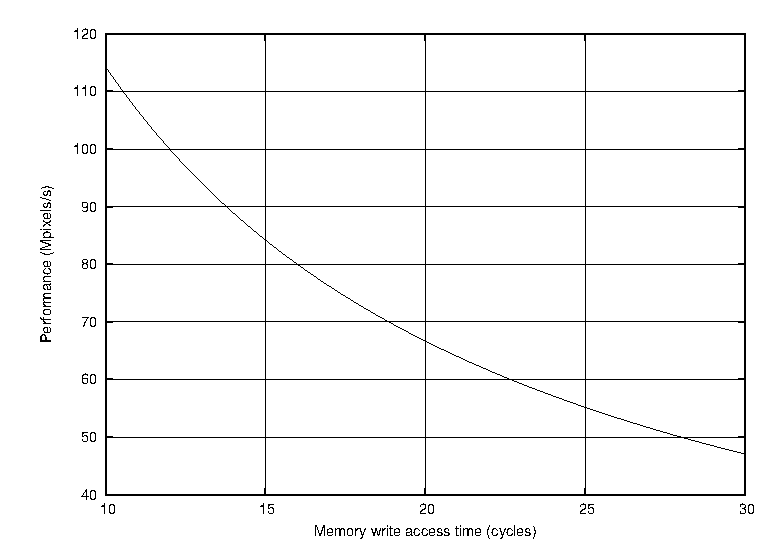
\includegraphics[height=50mm]{thwbufperf.eps}
  \end{figure}
}


\subsection{Performance results}
\frame
{
  \frametitle{Performance results}
  \begin{itemize}
  \item Depends on cache hit rate.
  \item Enough performance for MilkDrop in 640x480 30fps.
  \end{itemize}
  \begin{figure}[H]
  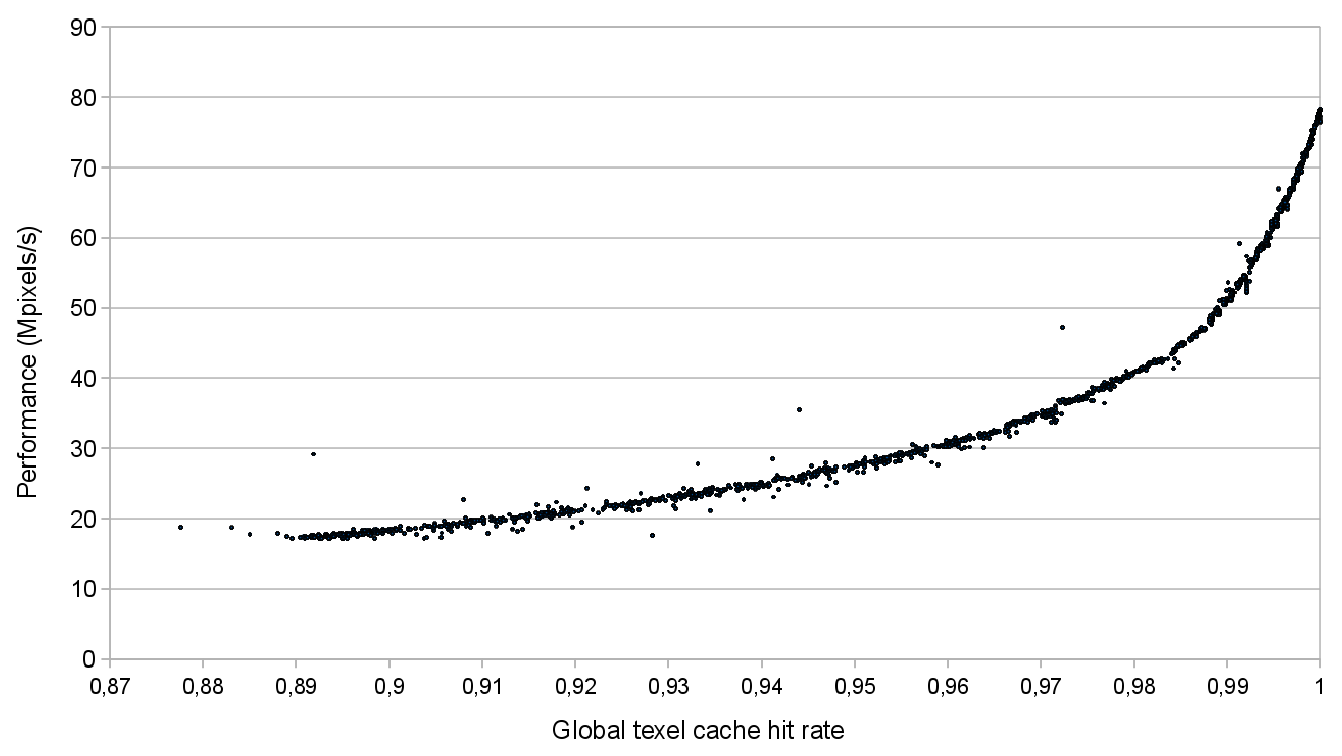
\includegraphics[height=50mm]{tmuresult.eps}
  \end{figure}
}

\section{Generating texture coordinates}
\subsection{The problem}
\frame
{
  \frametitle{The problem}
  \begin{itemize}
  \item Intensive floating point processing, for each vertex.
  \item At least $\approx 58$ million operations per second needed.
  \item Cannot be met with an in-order FPU at 100MHz in FPGAs (CPI $< 1.73$).
  \item We need parallelism.
  \end{itemize}
}

\subsection{Levels of parallelism}
\frame
{
  \frametitle{Levels of parallelism}
  \begin{itemize}
  \item Two approaches:
  \begin{itemize}
  \item Vertex-level parallelism.
  \item Instruction-level parallelism.
  \end{itemize}
  \item Vertex-level parallelism requires more on-chip storage for temporary values.
  \item Instruction-level parallelism is potentially slower.
  \item The two approaches are not mutually exclusive.
  \item We focused on instruction-level parallelism only (simpler).
  \end{itemize}
}

\subsection{Instruction-level parallelism}
\frame
{
  \frametitle{Instruction-level parallelism}
  \begin{itemize}
  \item Out-of-order execution.
  \item Relatively expensive and complex hardware structures.
  \item We avoid them with instructions statically scheduled by the compiler.
  \begin{itemize}
  \item like VLIW architectures.
  \end{itemize}
  \item Works well, because:
  \begin{itemize}
  \item all delays are known (negligible memory accesses).
  \item no control hazards.
  \end{itemize}
  \end{itemize}
}

\subsection{Results}
\frame
{
  \frametitle{Results}

  \begin{tabular}{|l|l|l|l|l|l|}
  \hline
  \textbf{Patch} & \textbf{Instructions} & \textbf{Cycles} & \textbf{CPI} \\
  \hline
  Default & 192 & 259 & 1.35 \\
  \hline
  The Tunnel & 208 & 286 & 1.38 \\
  \hline
  Warp of Dali 1 & 220 & 292 & 1.33 \\
  \hline
  Digital Flame & 216 & 293 & 1.36 \\
  \hline
  Wormhole Pillars & 231 & 326 & 1.41 \\
  \hline
  \end{tabular}
  \begin{itemize}
  \item We needed CPI $< 1.73$.
  \item Success!
  \end{itemize}
}

\section{Conclusion}
\frame
{
  \frametitle{Conclusion}
  \begin{itemize}
  \item We have developed a working MilkDrop rendering program for the SoC.
  \begin{itemize}
  \item proof of concept
  \end{itemize}
  \item Further development
  \begin{itemize}
  \item Interfaces support: video input, DMX, MIDI, USB ...
  \item Operating system support.
  \item End user application.
  \item ``Packaged'' device.
  \end{itemize}
  \item Further research
  \begin{itemize}
  \item Out-of-order memory subsystem.
  \item Texture mapping unit prefetching.
  \item High level synthesis.
  \end{itemize}
  \end{itemize}
}

\frame
{
  \frametitle{Thank you for your attention}
  \begin{itemize}
  \item Web: \url{http://www.milkymist.org}
  \item Mailing list: devel [AT] lists [DOT] milkymist [DOT] org
  \end{itemize}

  \begin{center}
  \framebox[100mm][c]{Demonstration \& questions}
  \end{center}
}

\end{document}
